\documentclass[12pt,a4paper]{article}
\pagestyle{plain}
\usepackage{fullpage}
\usepackage[english]{babel}
\usepackage{enumerate}

%equations
\usepackage[fleqn]{amsmath}
\numberwithin{equation}{section}

%figures
\usepackage[dvips]{graphicx}
\graphicspath{{./images/}}
\numberwithin{figure}{section}

%excercises
\newcounter{Exercise}
\setcounter{Exercise}{1}
\usepackage[dvipsnames]{xcolor}
\usepackage{framed}
\definecolor{shadecolor}{gray}{0.9}
\usepackage{caption}

%tables
\numberwithin{table}{section}

%specials
\usepackage{textcomp} %special (greek) characters as text
%\usepackage{pstricks} %
%\usepackage{ifthen} %
%\usepackage{calc} %
%\usepackage{isotope}
\usepackage{hyperref}
\usepackage[bottom]{footmisc} %footnote below figure
\usepackage{footnpag}%number footnotes per page
\usepackage{nicefrac}%fractions with slash


%document details
\author{N.G. Schultheiss \\ translated and adapted by K. Schadenberg}
\date{}
\title{de Broglie}


\begin{document}
\maketitle

\section{Introduction}
This module follows the module `HiSPARC Detector Plate' and is followed by `Fluorescence'. The first lesson letter of this series explained what happens with the light created inside the detector plate. `Fluorescence' describes in detail how this light is created and what determines the colour of light. This text briefly explains what determines the colour of light and the internal structure of atoms. 

\section{Particles or Waves}
In the 17th century two great minds of science were in disagreement over the fundamental properties of light. Newton argued that light was a particle, while Huygens stated that is was a wave. Both were able to accurately describe the behaviour of light.\footnote{See `Mirrors' for more details.} At the beginning of the 20th century Louis de Broglie offered a solution to this problem with his theory about matter waves (or de Broglie waves). Today one of the key concepts of quantum mechanics is the wave-particle duality. De Broglie, together with Max Planck, Arthur Compton, Niels Bohr, and many others laid the foundations for the theory.
The following equations are known as the de Broglie relations:
\begin{align}
\lambda &= \frac{h}{p} \label{eq:broglie_1} \\ 
f &= \frac{E}{h} \label{eq:broglie_2}
\end{align}
In these equations $\lambda$ is the wavelength and $p$ is the momentum of a particle, $h$ is the Planck constant ($6.626 \cdot 10^{-34}$ ~J~$\cdot$~s). The momentum $\textbf{p}$ can be calculated using the mass $m$ and the velocity $\textbf{v}$ of the particle:
\begin{equation}
\textbf{p}= m \cdot \textbf{v} \label{eq:momentum} 
\end{equation}
\textbf{p} and \textbf{v} are printed using bold letters to indicate that they not only have a magnitude (a size or number) but also a direction. When calculating the de Broglie wavelength the direction of the momentum is not important. One only needs to know `how large' the momentum is (i.e. the number). This is represented by printing $p$ not using a bold font.\footnote{Most printed texts use bold lettering to denote vectors. However, when writing using pen and paper it can be quite difficult to write bold letters, therefore a line can be drawn below (or above in some cases) the letter to indicate that it is a vector: \underline{p}.} Remember to use SI units in all equations.

\begin{shaded} \textbf{Exercise \theExercise \stepcounter{Exercise}} : Use the SI unit for mass $m$ and velocity $v$ to derive the unit for momentum $p$. \end{shaded}
\begin{shaded} \textbf{Exercise \theExercise \stepcounter{Exercise}} : The wavelength $\lambda$ has the unit [m]. Use this to verify the given unit for the Planck constant. \end{shaded}

De Broglie's idea that light behaves both as a wave and a particle let him to wonder if this was also true for other particles. Do electrons, which were seen as particles, also show wave like characteristics? The answer was yes as was shown by what is now voted as the most beautiful physics experiment: Young's double-slit experiment applied to the interference of single electrons.\footnote{See \url{http://www.youtube.com/watch?v=ZJ-0PBRuthc} for a brief movie of this experiment.} Using the notion of electrons as waves and particles, de Broglie was able to explain the fixed electron orbits of atoms. In the next section we will take a closer look at the electron orbits in a hydrogen atom.

\section{The hydrogen atom}
The hydrogen atom is the simplest atom we know, it consists of a single proton around which a single electron orbits. But even this simple atom can be difficult to describe using equations and mathematics. In the following description we will assume that both the electron and the proton have the smallest electrical charge possible, albeit with opposite signs. This charge is called the elementary charge $e$, $e=1.602176565 \cdot 10^{-19}$~C.

Because the proton and electron have (opposite) charges they are both influenced by electrical forces. The strength of an electrical force can be calculated using Coulomb's law:
\begin{equation}
F_{el} = \frac{q_1 q_2}{4 \pi \epsilon_0 r^2} \label{eq:force_elec} 
\end{equation}
The electrical force $F_{el}$ between two charged particles $q_1$ and $q_2$ is dependent on the strength of the charges in Coulombs (C) and the distance between the two charges $r$, $\epsilon_0$ is the vacuum permittivity. 

\begin{shaded} \textbf{Exercise \theExercise \stepcounter{Exercise}} : Using equation~\ref{eq:force_elec} one can easily calculate the forces on the proton and electron inside the hydrogen atom once the distance between the two is known. How do these forces change when we look at a helium atom? Remember that a helium atom has two protons inside the nucleus. Does the force on a single electron change if we were to look at a He$^+$ ion instead of a neutral atom?\end{shaded}

If the electron were standing still it would be accelerated by this electrical force and start to move towards the proton. However, the electron does not stand still, it has a certain speed. The force between the proton and electron causes the electron to move in a circular orbit around the proton. The centripetal acceleration needed to maintain a certain orbit can be calculated using the following equation:
\begin{equation}
F_{centripetal} = \frac{m v^2}{r} \label{eq:force_cent} 
\end{equation}
The electron orbits around the proton (because the proton is much heavier) therefore the mass $m$ is the mass of the electron and $v$ its speed. The radius of the orbit is denoted with the $r$. Which force is responsible for the centripetal acceleration? The only force present: the electrical force:
\begin{equation}
\frac{m v^2}{r} = \frac{q_1 q_2}{4 \pi \epsilon_0 r^2} \label{eq:force_elec_centr} 
\end{equation}

According to de Broglie the electron has a certain wave length. To use the de Broglie relations to calculate this wave length, we first need to calculate the momentum of the electron using its speed, which we can then use to calculate the wave length:
\begin{equation}
\frac{\left( {m v}\right) ^2}{m} = \frac{q_1 q_2}{4 \pi \epsilon_0 r} \Rightarrow \frac{p^2}{m}=\frac{q_1 q_2}{4 \pi \epsilon_0 r} \Rightarrow \frac{h^2}{m \lambda^2} = \frac{q_1 q_2}{4 \pi \epsilon_0 r} \label{eq:force_elec_centr_2} 
\end{equation}

There must be a integer number of waves in the orbit of the electron, otherwise the electron wave will extinguish itself. In other words: The electron wave must be a standing wave around the proton, the nodes and anti-nodes of the wave do not move:
\begin{equation}
n \lambda = 2 \pi r \Rightarrow \lambda = \frac{2 \pi r}{n} \label{eq:number_of_waves} 
\end{equation}
We obtain the wave length by substituting equation~\ref{eq:number_of_waves} in equation~\ref{eq:force_elec_centr_2}:
\begin{equation}
\left( \frac{n}{2 \pi r}\right)^2 \frac{h^2}{m} = \frac{q_1 q_2}{4 \pi \epsilon_0 r} \Leftrightarrow \frac{n^2 h^2}{4 \pi^2 r m} = \frac{q_1 q_2}{4 \pi \epsilon_0 r} \label{eq:number_of_waves_centr2} 
\end{equation}
\begin{equation}
r=\frac{\epsilon_0 n^2 h^2}{\pi m q_1 q_2} \label{eq:result_r} 
\end{equation}
The radius of the orbit can be calculated by inserting the various constants. The orbit with $n=1$:
\begin{equation}
r_1=\frac{8.854187817 \cdot 10^{-12} ~ 1^2 \left( 6.626069 \cdot 10^{-34} \right)^2 }{3.14159 ~ 9.11 \cdot 10^{-31} \left( 1.602176462 \cdot 10^{-19} \right)^2 } \approx 0.53 \cdot 10^{-10}~\mbox{m} \label{eq:result_r_1} 
\end{equation}

\begin{shaded} \textbf{Exercise \theExercise \stepcounter{Exercise}} : Explain how the result of equation~\ref{eq:result_r_1} also gives us the size of the hydrogen atom.\end{shaded}

In equation~\ref{eq:result_r_1} we calculated the radius for the orbit $n=1$, of course there are also orbits with $n=2$, $n=3$, etc. Every atom has a fixed series of electron orbits, with fixed radii. Because the orbits are fixed, the energy differences between these orbits are also fixed.

An atom can absorb energy by absorbing a photon, in a similar fashion it can expel energy by emitting a photon. The energy of a photon:
\begin{equation}
E_{photon} = h\nu = \frac{hc}{\lambda_{photon}} \label{eq:E_photon}
\end{equation}
$\nu$ denotes the frequency of the photon. Because the energy transitions of the electrons are fixed, so are the possible emitted and absorbed photons. This allows one the recognise an atom by the light it absorbs or emits.

\begin{figure}\begin{center}
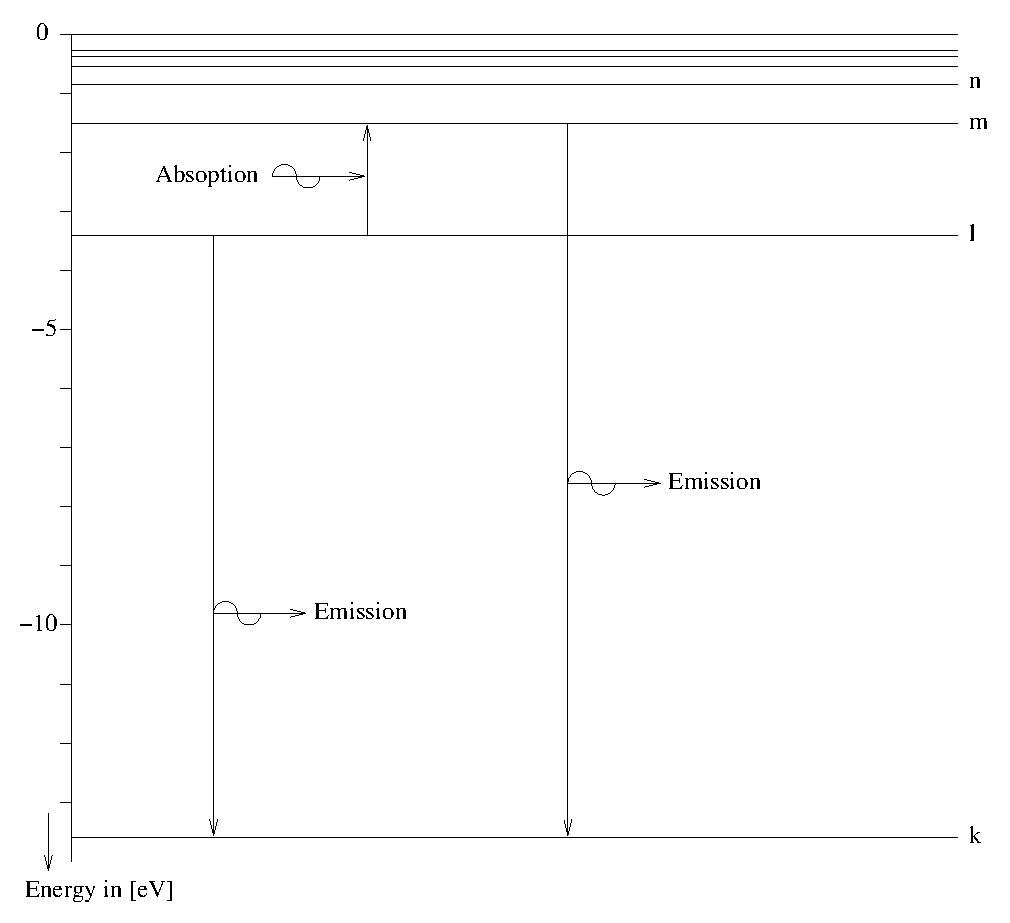
\includegraphics[scale=0.8]{hydrogen.eps}
\caption{Energy levels of an electron in a hydrogen atom.}\label{fig:shower_angles}
\end{center}\end{figure}

\begin{shaded} \textbf{Exercise \theExercise \stepcounter{Exercise}} : Explain in your own words why and how you can recognise atoms by their absorption or emission of light. \end{shaded}

\section{Absorption lines}
When two charges are separated in free space by an infinitely large distance they will feel no force. Because this proposition is true for all charges we state that the electrical energy of these two charges is equal to 0~eV. With this statement electrical energy is defined unambiguously.
When the two charges move toward each other there will be a force (now there is a finite distance). We now have a force which acts upon a body which is moving in the direction of the force: Work.
\begin{equation}
W = \textbf{F} \textbf{d}  \label{eq:work}
\end{equation}
In this equation \textbf{d} is the distance travelled.

The electrical force in equation~\ref{eq:force_elec} is a function of distance ($r$). We use this to calculate the work done:
\begin{equation}
W = \frac{q_1 q_2}{4 \pi \epsilon_0 r^2} d \cdot \cos(\alpha) \label{eq:work_elec}
\end{equation}
Here we changed the distance travelled from a vector \textbf{d} to a scalar $d$ multiplied with the angle between the force and the direction of travel. If the force and path are aligned parallel the equation simplifies into:
\begin{equation}
W = \frac{q_1 q_2}{4 \pi \epsilon_0 r^2} d \label{eq:work_elec_2}
\end{equation}

We want to solve this equation for $W$. The distance travelled $d$ is the distance between two orbits, or in other words the difference between the two radii ($dr$). Note that the strength of the electrical force changes with the distance between the electron and proton!
\begin{equation}
W = \int \frac{q_1 q_2}{4 \pi \epsilon_0} \frac{1}{r^2} dr \Leftrightarrow W = \frac{q_1 q_2}{4 \pi \epsilon_0} \int \frac{1}{r^2} dr \label{eq:work_elec_int}
\end{equation}
\begin{equation}
W_{start \rightarrow end} = - \frac{q_1 q_2}{4 \pi \epsilon_0} \left( \frac{1}{r_{end}} - \frac{1}{r_{start}}\right) = \frac{q_1 q_2}{4 \pi \epsilon_0} \left( \frac{1}{r_{start}} - \frac{1}{r_{end}}\right) \label{eq:work_elec_end_start}
\end{equation}
Equation~\ref{eq:result_r} gives us the allowed radii. Applying this to the previous equation:
\begin{equation}
W_{start \rightarrow end} = \frac{q_1 q_2}{4 \pi \epsilon_0} \left( \frac{\pi m q_1 q_2}{ \epsilon_0 n_{1}^2 h^2} - \frac{\pi m q_1 q_2}{\epsilon_0 n_{2}^2 h^2}\right)  \label{eq:work_elec_end_start_r}
\end{equation}
\begin{equation}
W_{start \rightarrow end} = \frac{m q_{1}^2 q_{2}^2}{4 \epsilon_{0}^2 h^2} \left( \frac{1}{n_{1}^2} - \frac{1}{n_{2}^2}\right) \label{eq:work_elec_end_start_r_simplified}
\end{equation}

A part of the electrical energy is converted into kinetic energy. Because the speed of the electron lies far below the speed of light the following relation holds:
\begin{equation}
E_{kin} = \frac{1}{2} mv^2 = \frac{1}{2} \frac{p^2}{m} = \frac{1}{2} \frac{q_1 q_2}{4 \pi \epsilon_0 r} = \frac{1}{2} \frac{q_1 q_2}{4 \pi \epsilon_0} \frac{\pi m q_1 q_2}{\epsilon_0 n^2 h^2}=\frac{m q_{1}^2 q_{2}^2}{8 \epsilon_{0}^2 n^2 h^2}% \left( \frac{1}{n_{1}^2} - \frac{1}{n_{2}^2} \right) 
\label{eq:E_kin}
\end{equation}

When the orbit of the electron changes, its (electrical) potential energy also changes:
\begin{equation}
E_{pot}=- \frac{1}{4 \pi \epsilon_0} \frac{q_1 q_2}{r} = - \frac{m q_{1}^2 q_{2}^2}{4 \epsilon_{0}^2 n^2 h^2} \label{eq:pot}
\end{equation}
The total amount of energy of the electron is the sum of the potential and kinetic energy and is a function of the orbit number:
\begin{equation}
E_{n} = \frac{m q_{1}^2 q_{2}^2}{8 \epsilon_{0}^2 n^2 h^2} - \frac{m q_{1}^2 q_{2}^2}{4 \epsilon_{0}^2 n^2 h^2} = - \frac{m q_{1}^2 q_{2}^2}{8 \epsilon_{0}^2 h^2} \frac{1}{n^2} \label{eq:E_tot}
\end{equation}
During a downward transition of an electron (the electron goes from an excited or higher energy state towards a lower one) a part of the electron's potential energy is converted into kinetic energy and at the same time a photon is created.

%\begin{flalign}
%E_{kin} + E_{pot} + E_{photon} \Leftrightarrow E_{photon} = E_{pot} - E_{kin}
%\label{eq:trans_down}
%\end{flalign}

\begin{equation}
E_{photon} = h \nu = \frac{m q_{1}^2 q_{2}^2}{8 \epsilon_{0}^2 h^2}\left( \frac{1}{n_{1}^2} - \frac{1}{n_{2}^2} \right) \label{eq:E_photon2}
\end{equation}
\begin{equation}
\frac{1}{\lambda} = \frac{m q_{1}^2 q_{2}^2}{8 \epsilon_{0}^2 c h^3} \left( \frac{1}{n_{1}^2} - \frac{1}{n_{2}^2} \right) = R \left( \frac{1}{n_{1}^2} - \frac{1}{n_{2}^2} \right) \label{eq:lambda_rydberg}
\end{equation}
$R$ is the Rydberg constant. Equation~\ref{eq:lambda_rydberg} can be used to calculate the wavelength of the emitted photon. During an upward transition of an electron (from a lower energy level to a higher one) the atom absorbs a photon. The atom is now in an excited state.

\end{document}

